\documentclass{article}

\usepackage{float}
\usepackage{amsmath}
\usepackage{amsfonts}
\usepackage{amssymb}
\usepackage{graphicx}
\usepackage[margin=1in]{geometry}

\usepackage[backend=biber, style=alphabetic, sorting=ynt]{biblatex}
  
\title{Week 5 - Homework}
\author{Artur Topal, S5942128}
\date{\today}

\begin{document}

\maketitle

\begin{center}
  \textbf{TA}: Hanna, grp\_356739\_6
\end{center}

\pagebreak

\section{ Problem H1 } 

Use spherical coordinates $(r, \theta, \phi)$ with the origin in the center of Earth, where $\phi$ is azimuthal angle. Then, since altitude $h$ is measured from the surface of Earth, in terms of $r$ it is $h=r-R$ and we should integrate $r$ from $r=R$ to $r=\infty$. The volume density function is then $\rho(h) = \rho_0 e^{-\frac{h}{H}} = \rho(r) = \rho_0 e^{-\frac{r-R}{H}}$. Earth is a perfect sphere, therefore spherical symmetry is present. Thus, $\int_{\Omega_r} d\Omega_r = 4\pi$, where $d\Omega_r = \sin(\theta) d\theta d\phi$. The mass of the atmosphere can be computed as follows:

\begin{equation*}
M = \int_{R}^{\infty} \rho_0 e^{-\frac{r-R}{H}} 4\pi r^2 dr = 4\pi \rho_0 \int_{R}^{\infty} r^2 e^{-\frac{r-R}{H}} dr
\end{equation*}

Substitute $u = \frac{r- R}{H}$, $du = \frac{dr}{H}$, $r = uH + R$, and $dr = Hdu$, where $u$ is dimensionless.

\begin{equation*}
M = 4\pi \rho_0 \int_{0}^{\infty} (uH + R)^2 e^{-u} Hdu
\end{equation*}
\begin{equation*}
M = 4\pi \rho_0H \int_{0}^{\infty} (uH)^2 e^{-u} du + 4\pi \rho_0H \int_{0}^{\infty} (R)^2 e^{-u} du + 4\pi \rho_0H \int_{0}^{\infty} 2uHR e^{-u} du
\end{equation*}

\begin{equation} \label{eq:mass_uneval}
M = 4\pi \rho_0H^3 \int_{0}^{\infty} u^2 e^{-u} du + 4\pi \rho_0HR^2 \int_{0}^{\infty} e^{-u} du + 8\pi \rho_0H^2R \int_{0}^{\infty} u e^{-u} du
\end{equation}

Compute the integrals: 
\begin{equation*}
  \int_0^\infty e^{-u} du = -e^{-u} |_0^\infty = "-\frac{1}{e^\infty}" + \frac{1}{e^0} = 1
\end{equation*}

\begin{equation*}
  \int_0^\infty u e^{-u} du = -ue^{-u}|_0^\infty + \int_0^{\infty} e^{-u} du = 0 + 1 = 1
\end{equation*}

\begin{equation*}
  \int_0^\infty u^2 e^{-u} du = -u^2e^{-u}|_0^\infty + 2\int_0^{\infty} ue^{-u} du = 0 + 2 \times 1 = 2
\end{equation*}

Substitute the integrals back into Eq.~\eqref{eq:mass_uneval}.

\begin{equation*}
M = 4\pi \rho_0H^3 \times 2 + 4\pi \rho_0HR^2 \times 1 + 8\pi \rho_0H^2R \times 1 = 4 \pi H \rho_0 (2H^2 + R^2 + HR)
\end{equation*}

Check using dimensional analysis:
\begin{equation*}
  [M] = [H] [\rho_0] ([H^2] + [R^2] + [HR]) = m \frac{kg}{m^3} (m^2 + m^2 + m^2) = kg
\end{equation*}

Plug in the numbers (note, that $R$, $H$ were in $km$):
\begin{equation*}
  M = 4\pi \times 10 \times 1.2 (2 \times 10^2 + 6378^2 + 10 \times 6378) \times 1000^2 \approx 6.1 \times 10^{15} kg
\end{equation*}

\section{ Problem H2 }

\textbf{a)} Find the moment of inertia of a solid sphere with uniform volume velocity $\rho$. Orient the Cartesian coordinate system in a way that $z$ axis coincides with the rotation axis of the sphere (see Fig.\ref{fig:2a}).

Then,
\begin{equation*}
  I_{sphere} = \int_{sphere} a^2 dm = \rho \int_{sphere} a^2 dV
\end{equation*}
where $a$ is the distance from $dV$-point to the rotation axis. According to Fig.\ref{fig:2a}, it is $r\sin(\theta)$ 

\begin{figure}[H]
  \centering
  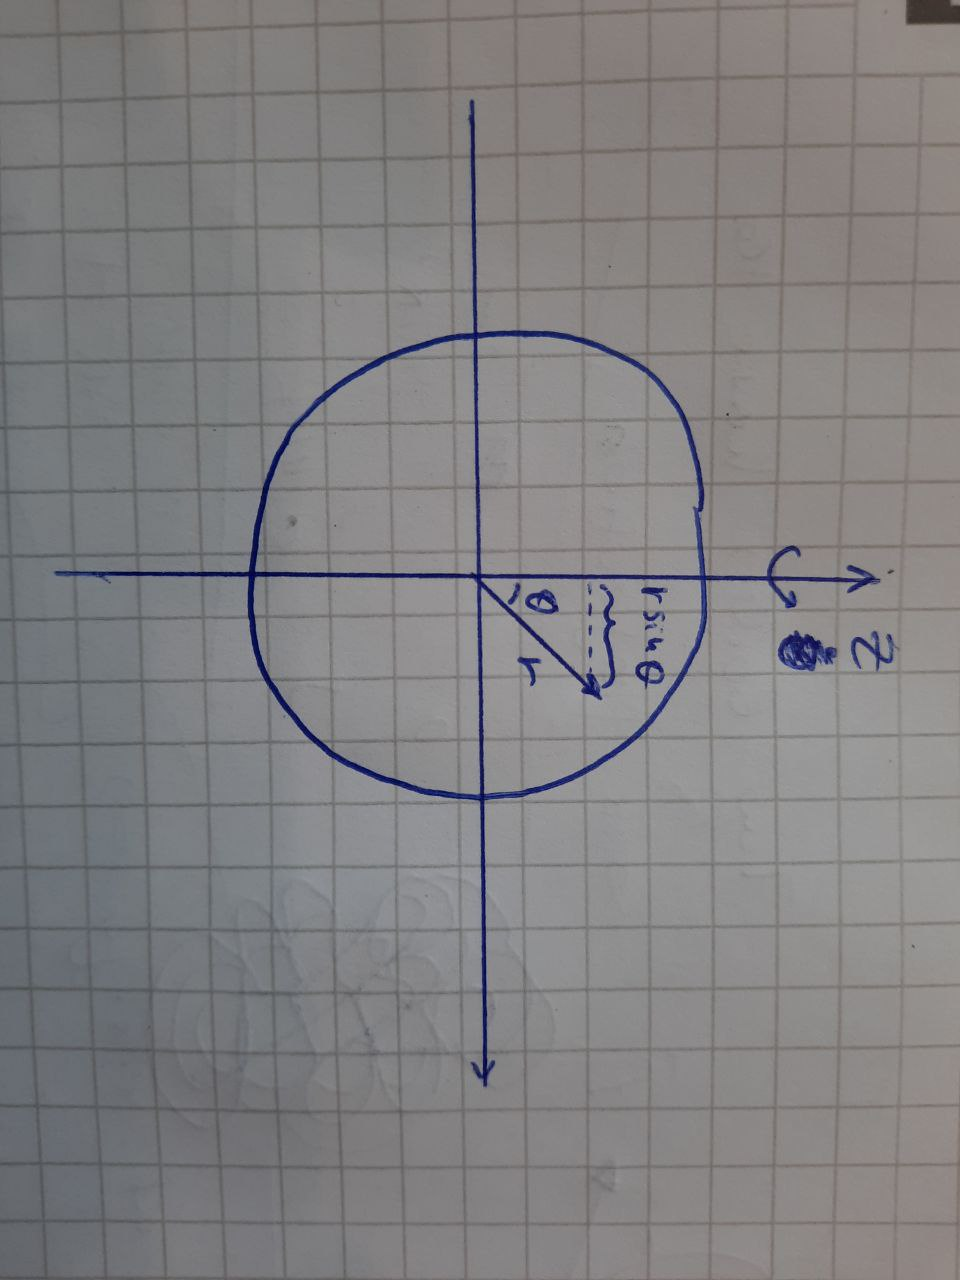
\includegraphics[width=0.3\textwidth, angle=90]{calculus/W5/img/2a}
  \caption{Spherical coordinates}
  \label{fig:2a}
\end{figure}

Thus,
\begin{equation*}
  I_{sphere} = \rho \int_{r=0}^{R} \int_{\theta = 0}^{\pi} \int_{\phi = 0}^{2\pi} (r\sin(\theta))^2 r^2 \sin(\theta) d\phi d\theta dr = \rho \int_{r}^{R} r^4 dr  \int_{\theta}^{\pi} \sin(\theta)^3 d\theta \int_{0}^{2\pi} d\phi = \rho \times \frac{R^5}{5} \times 2\pi \times \frac{4}{3} = \frac{8\pi \rho R^5}{15}
\end{equation*}
where
\begin{equation*}
  \int_{0}^{\pi} \sin(\theta)^3 d\theta = (-\frac{1}{3} \cos(\theta) \sin(x)^2 + \frac{2}{3} (-cos(\theta)) )_{0}^\pi = \frac{4}{3}
\end{equation*}

In \textbf{c)}, I will need the inertia moment in terms of mass. $\rho = \frac{m}{\frac{4}{3} \pi R^3} = \frac{3m}{4\pi R^3}$. Thus $I_{sphere}(m) = \frac{8\pi R^5}{15} \times \frac{3m}{4\pi R^3} = \frac{2}{5}mR^2$.

\begin{equation*}
  R_g = \sqrt{ \frac{\frac{2}{5}mR^2}{m} } = R \sqrt{\frac{2}{5}}
\end{equation*}
  
Answer: $R_g = R \sqrt{\frac{2}{5}}$ and $I_{sphere}(m) = \frac{2}{5}mR^2$

\textbf{b)}
Here, the strategy is the same but I use cylindrical coordinates instead of spherical ones.

\begin{figure}[H]
  \centering
  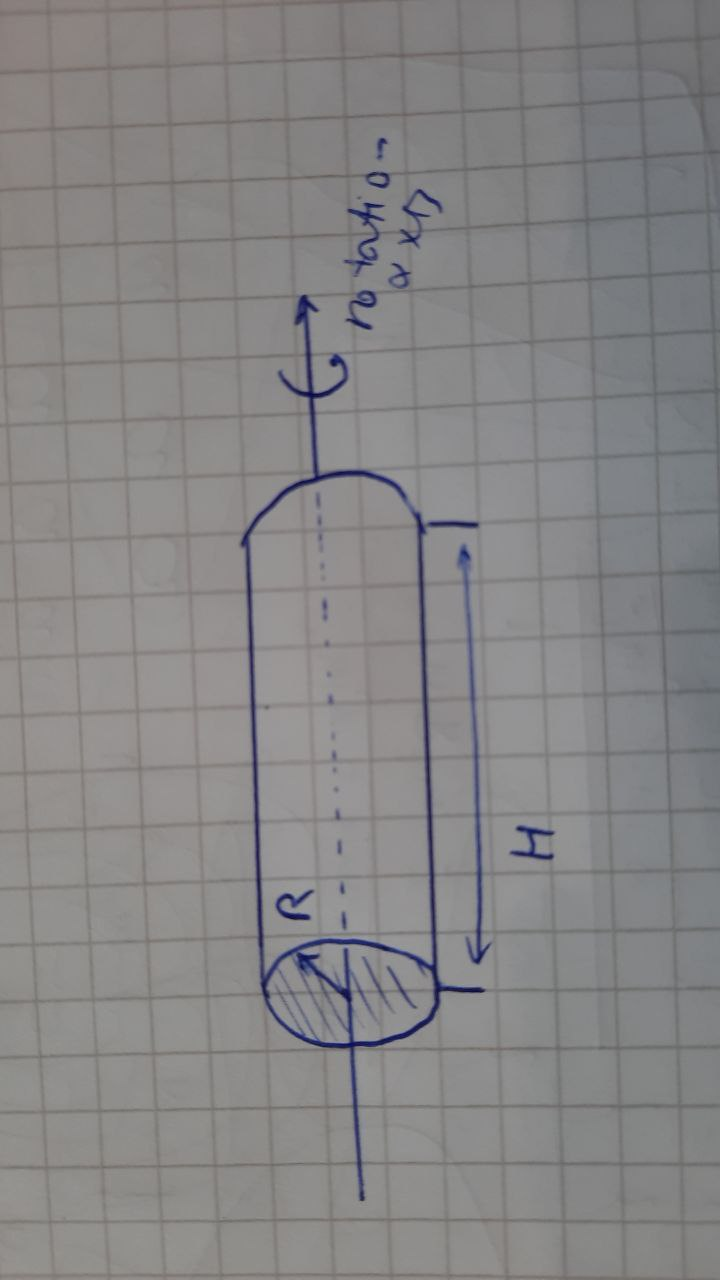
\includegraphics[width=0.3\textwidth, angle=-90]{calculus/W5/img/2b}
  \caption{Cylindrical coordinates}
  \label{fig:2b}
\end{figure}

\begin{equation*}
  I_{cylinder} = \rho \int_{cylinder} r^2 dV = \rho \int_{r=0}^{R} \int_{\theta=0}^{2\pi} \int_{z=0}^{H} r^2 r dr d\theta dz = \rho \int_{0}^R r^3 dr \int_{0}^{2\pi} d\theta \int_{0}^{H} dz
\end{equation*}

\begin{equation*}
  \Rightarrow I_{cylinder} = \rho \frac{R^4}{4} 2\pi H = \frac{\pi H\rho R^4}{2}
\end{equation*}

As in \textbf{a)}, I will also provide a formula for the inertia moment in terms of the mass of the cylinder. ($\rho = \frac{m}{\pi R^2 H}$)
\begin{equation*}
  I_{cylinder}(m) = \rho = \frac{m}{\pi R^4 H} \frac{R^2}{2} \pi H = \frac{1}{2} mR^2
\end{equation*}

\begin{equation*}
  R_g = \sqrt{\frac{1/2mR^2}{m}} = R/\sqrt{2}
\end{equation*}
  
Answer: $R_g = R/\sqrt{2}$, $I_{cylinder}(m) = \frac{1}{2} mR^2$.

\textbf{c)}
\begin{figure}[H]
  \centering
  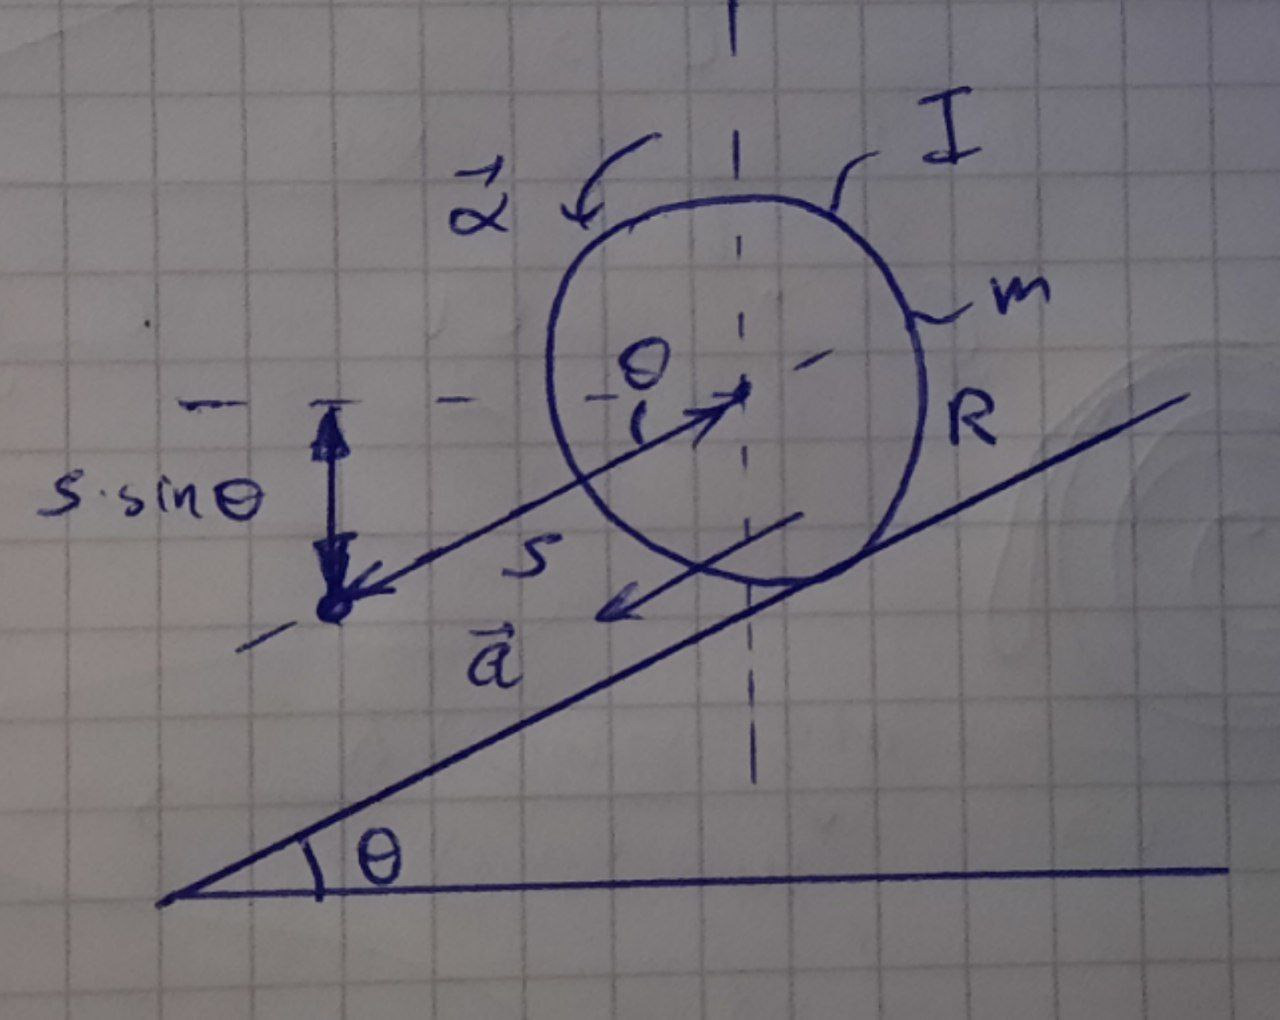
\includegraphics[width=0.3\textwidth]{calculus/W5/img/2c}
  \caption{An object and a slope}
  \label{fig:slope}
\end{figure}

Both the cylinder and the ball have the same mass $m$ if $H$ is $4/3R$. Since both objects look the same under $z$-projection, Fig. \ref{fig:slope} represents both objects. As the object travels distance $s$ down the slope, conservation of energy is:
\begin{equation*}
  mgs \sin(\theta) = \frac{1}{2}mv^2 + \frac{1}{2}I\omega^2
\end{equation*}
There is no slipping $\Rightarrow \omega = \frac{v}{R}$, where $R$ is the radius of the object. Thus,
\begin{equation} \label{eq:velocity}
  2mg s \sin(\theta) = mv^2 + \frac{Iv^2}{R^2} \Rightarrow v^2 = \frac{2mgs \sin(\theta)}{m + \frac{I}{R^2}} \Rightarrow v^2 = g\frac{2s\sin(\theta)}{1 + \frac{I}{mR^2}} 
\end{equation}
where $C =g\frac{2\sin(\theta)}{1 + \frac{I}{mR^2}} = const$

Differentiate both sides of Eq.~\eqref{eq:velocity}.
\begin{equation*}
  \frac{d}{dt} v^2 = C \frac{ds}{dt} \rightarrow 2v \frac{dv}{dt} = Cv \Rightarrow a = C/2
\end{equation*}

Therefore,
\begin{equation*}
  a = \frac{g\sin(\theta)}{1 + \frac{I}{mR^2}}
\end{equation*}

\begin{equation*}
  \Rightarrow a_{sphere} = \frac{g\sin(\theta)}{1 + \frac{\frac{2mR^2}{5}}{mR^2}} = 5/7g\sin(\theta)
\end{equation*}
And
\begin{equation*}
  \Rightarrow a_{cylinder} = \frac{g\sin(\theta)}{1 + \frac{\frac{mR^2}{2}}{mR^2}} = 2/3g\sin(\theta)
\end{equation*}

$2/3 > 5/7 \Rightarrow$ Acceleration of the cylinder is bigger than the sphere, so the cylinder will reach the bottom first. 

\end{document}
